\cotefile{157-4}
\scanpage{148}\mspage{22}
de cardinal majoré par
\[
\underset{\begin{gathered}\text{\unsure{nb de ces|nb des|nb de classes}}\\\text{syst. inductifs}\\\text{dans }\uuline{M}^{\pi},\ \unsure{?|\text{à}}\\\text{isom près}\end{gathered}}{
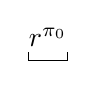
\begin{tikzpicture}[baseline=(a.base)]
\node[inner sep=0pt] (a) {$r^{\pi_0}$};
\draw ([yshift=-2pt]a.south west)--++(0,-3pt)-|([yshift=-2pt]a.south east);
\end{tikzpicture}}
\cdot
\underset{\begin{gathered}\text{\unsure{nb des|nb de}}\\\text{flèches d'un}\\\text{tel syst. ind.}\\\text{dans }X\end{gathered}}{
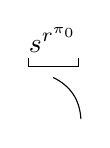
\begin{tikzpicture}[baseline=(b.base)]
\node[inner sep=0pt] (b) {$s^{r^{\pi_0}}$};
\draw ([yshift=-2pt]b.south west)--++(0,-3pt)-|([yshift=-2pt]b.south east);
\draw ([yshift=-9pt]b.south) to[bend left=30] ++(10pt,-15pt);
\end{tikzpicture}}
=s^{r^{\pi_0}}.
\]
Mais il faut maintenant faire varier $I$, à isom près, dans \unsure{la|le} cat des ens. ordonnés (\unsure{filtrants|filtrant} \unsure{etc|et}) de cardinal $\unsure{\le|\ge}\inserted{\lambda=}\unsure{r}^{\pi_0}\deleted{\unsure{\mathrm{card}\,I|\mathrm{card}}}$. On voit de suite que cet ensemble des classes d'isomorphie (qui peut s'interpréter comme un quotient d'\deleted{\unsure{l'|un}}\inserted{un certain} ens \unsure{de|des} \unsure{parties|relations} d'un ens. fixe $I_0$ de card $\lambda$) est de cardinal $\le2^\lambda$.
On trouve donc finalement
\[
\mathrm{card}\,\widetilde{M^r_{/X}}\le s^{(r^{\pi_0})}\cdot2^{(r^{\pi_0})}=s^{(r^{\pi_0})},
\]
sous condition que
\[
r\ge\mathrm{Sup}(\pi_1,C_0),\qquad s\ge\mathrm{Sup}(\pi_1,C_1).
\]
Il faut prouver l'inégalité similaire pour $\mathrm{card}\,\widetilde{\underline{\mathrm{Fl}}^r M}$ (3.9.). Or, \deleted{\unsure{le même calcul|le même cardinal|pour un cardinal}} pour \unsure{tt} $A,B$ dans $M^r$, on a si $r\ge\mathrm{Sup}(\pi_1,C_1)$
\[
\mathrm{card}\,\mathrm{Hom}_M(A,B)\le r^{(r^{\pi_0})}
\]
en vertu de (3.8) où on fait $s=r$, \unsure{on|et} \unsure{trouve|donc} que
\[
\begin{aligned}
\mathrm{card}\,
\underset{\deleted{\unsure{\mathrm{Fl}(M^r)|\mathrm{Fl}(M^r}\unsure{.}}}{
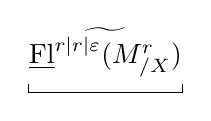
\begin{tikzpicture}[baseline=(c.base)]
\node[inner sep=0pt] (c) {$\widetilde{\underline{\mathrm{Fl}}^{\unsure{\deleted{r}|r|\varepsilon}}(M^r_{/X})}$};
\draw ([yshift=-2pt]c.south west)--++(0,-3pt)-|([yshift=-2pt]c.south east);
\end{tikzpicture}}
&\le\left(\mathrm{card}\,\widetilde{\unsure{M_{r/X}|M^r_{/X}}}\right)^2\cdot r^{(r^{\pi_0})}\\
&\le s^{(r^{\pi_0})}\cdot r^{(r^{\pi_0})}=s^{r^{\pi_0}},\\
&\text{si }s\ge r.
\end{aligned}
\]
% slanted
\margin{cf \unsure{cont.|corr.|cor.} p. 23}
(On va \unsure{regarder} plus bas le cas $s\le r^{\unsure{*|+}}$). C'est bien la formule (3.9.)
% archive sheet number: 147

\scanpage{149}\mspage{23}
Venons-en à la catégorie $M^r$ elle $=$. L'argument de la page 21 montre que l'ens des \inserted{classes d'isom} objets de $M^r$ indexés par un $I$ fixé, de cardinal $\le r^{\pi_0}$, comme
\[
\deleted{\unsure{X|A}}A=\underset{i}{\underset{\unsure{\mathrel{\text{---}}|\longrightarrow}}{\lim}}A_i
\quad\text{avec }A_i\in\mathrm{Filt}^{\pi_0},
\]
est de cardinal majoré par $r^{\pi_0}$ (si $r\ge C_0$). Si on fait varier $I$, on trouve \deleted{\unsure{la|le}} une majoration par $r^{\pi_0}\cdot2^{(r^{\pi_0})}=2^{(r^{\pi_0})}$.
On en \unsure{conclut} comme \unsure{tantôt|tantot} que \unsure{l'ens|bien} $\widetilde{\mathrm{Fl}\,M^r}$ est de cardinal majoré par
\[
\left(2^{(r^{\pi_0})}\right)^2\times r^{(r^{\pi_0})}\qquad(\text{si }r\ge\mathrm{Sup}(\pi_1,C_1)),
\]
donc par $r^{(r^{\pi_0})}$. Je dis qu'on a
\[
r^{(r^{\pi_0})}=2^{(r^{\pi_0})},
\]
en effet, on a $\ge$, et pour prouver $\le$, on note que $r<2^r$, donc
\[
r^{(r^{\pi_0})}\le(2^r)^{(\unsure{r}^{\pi_0})}=2^{r\cdot r^{\pi_0}}=2^{r^{\pi_0}},
\]
\unsure{\deleted{Cet argument}|Cet argument}
\deleted{\unsure{On a établi}}
\unsure{OK|ok} ! Cela établit donc 3.7.
\unsure{On a} en fait le
\uline{Lemme} \uline{3.2.} \unsure{Soient|Soit} $r$ un cardinal, $r'$ un cardinal $\ge r$. Alors on a
\[
r^{r'}=2^{r'}\qquad(=s^{r'}\text{ pour \unsure{tous|tout|ts} }2\le s\le r)
\]
\uline{Corollaire 1} \unsure{Soient|Soit} \deleted{$r\ge s\ge\mathrm{Sup}(\pi_1,C_1)$.} $r\ge\mathrm{Sup}(\pi_1,C_1)$, et $A,X\in\mathrm{Filt}^{\unsure{r|\pi}}$. Alors
\[
\mathrm{card}\,\mathrm{Hom}_M(A,X)\le2^{(r^{\pi_0})}
\qquad(=2^r\text{ si }r=2^c,\ \inserted{\text{avec}}\ c\unsure{\ge|>}\pi_0\unsure{)}
\tag*{(3.10),}
\]
On applique 3.8., \deleted{\unsure{car|au}} qui donne la majoration $r^{(r^{\pi_0})}$, et le lemme 3.2.

\deleted{\uline{Corollaire 2}}
On \unsure{note|voit} qu'on trouve la même majoration que pour le cardinal de $\widetilde{\underline{\mathrm{Fl}}(M^r)}$ \unsure{démonstration|détermination} (3.7)! $\unsure{D|\Delta}\unsure{=|\simeq}$ (3.9.) donne

\uline{Corollaire 2} Soit $r\ge\mathrm{Sup}(\pi_1,C_1)$, et $\unsure{\alpha|X}\in\mathrm{Ob}\,M^r$. Alors
\[
\mathrm{card}\,\widetilde{\underline{\mathrm{Fl}}(M^r_{/X})}\le2^{(\unsure{r}^{\pi_0})}
\qquad(=2^r\text{ si }r=2^c,\text{ avec }c\ge\pi_0).
\tag*{(3.11).}
\]
c'est donc la formule (3.9) pour $s\le r$, \unsure{laissée|laissé|laissee} en suspens.
% archive sheet number: 148

\scanpage{150}\mspage{24}
Revenons à la majoration cardinale des $X_\alpha(f)$, où $f:X\unsure{\mathrel{\text{---}}|\longrightarrow}Y$ \deleted{dans} ds $\mathrm{Fl}^{\unsure{s|B}}M$ i.e. $X,Y\in\mathrm{Filt}^s$. On suppose en plus $C_0\subset\deleted{\mathrm{Filt}}\mathrm{Fl}^rM$,
\deleted{\unsure{et}}
\[
\left\{\begin{aligned}
&C_0\subset\mathrm{Fl}^rM=\mathrm{Fl}\,M^r,\qquad(f:X\mathrel{\text{---}}Y)\in\mathrm{Fl}^sM\quad\text{i.e. }X,Y\in\mathrm{Filt}^s\\
&s\ge r
\end{aligned}\right.
\tag*{(3.10)}
\]
\deleted{\unsure{OBS} \unsure{pour} $C_0$, \inserted{\unsure{compté}} \unsure{mod.|modulo} \unsure{réun.|près|classes} \unsure{disjte|d'isom.}}
\[
\deleted{\mathrm{Card}\,\Delta(C_0,f)\le\mathrm{card}\,M^r_{/X}\times\mathrm{Card}\,M^r_{/Y},}
\]
Il y a une difficulté \unsure{idiote|ici}, c'est que \deleted{\unsure{de}} $M^r$ est équivalente à une petite catégorie, mais n'est pas elle-même petite. Même si $C_0$ ne \unsure{contenant|contenait} qu'une seule classe d'isomorphie de flèches de $M^r$, son cardinal pourrait être (pour $r$ fixé) arbitrairement élevé. Aussi dans ce qui suit, je \inserted{\unsure{dois|vais}} supposer \deleted{que le} \inserted{la condition} \deleted{\unsure{nb|est} \unsure{d'éléments|d'ailleurs} \unsure{cardinal} de \unsure{C|C_0}} de ``non \unsure{pléthoricité|pléthorité}'' cardinale pour $C_0$
\[
\begin{aligned}
&\forall i\in C_0,\ \deleted{\unsure{l'ens|désignant}}\inserted{\text{désignant}}\ \text{par }C_0(i)\text{ l'ens des}\\
&\deleted{\unsure{d'}}i'\in C_0\text{ telles que }i\simeq i'\text{ dans }\mathrm{Fl}\,M,\ \text{j'impose}\\
&\text{que}\quad\mathrm{card}\,C_0(i)\le2^{(r^{\pi_0})}\quad\text{(ce qui est \inserted{aussi}}\\
&\text{\inserted{visiblement la} majoration pour le cardinal de }\widetilde{\underline{\mathrm{Fl}}^rM}=\widetilde{\underline{\mathrm{Fl}}\,M^r})
\end{aligned}
\tag*{\unsure{(3.1b)|(3.11)}}
\]
\margin{$\deleted{\mathrm{card}}\inserted{\mathrm{card}\,C_0\le}\left(2^{(r^{\pi_0})}\right)^2=\mathrm{card}\,2^{r^{\pi_0}}$.}
Cela \unsure{entraîne|entraine} donc que l'on \unsure{a}
\[
\mathrm{card}\,C_0\le2^{(r^{\pi_0})},
\tag*{(3.12)}
\]
qui est équivalente à (3.1b) (moyennant $C_0\subset\mathrm{Fl}^rM$, postulé dans (3.10)).
Il s'ensuit \inserted{par (3.8)} que l'on a
\[
\mathrm{card}\,\Delta(C_0,f)\le
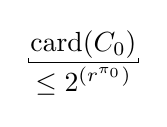
\begin{tikzpicture}[baseline=(t.base)]
\node[inner sep=1pt] (t) at (0,0) {$\mathrm{card}(C_0)$};
\draw (-0.7,-0.18)--(-0.7,-0.23)--(0.7,-0.23)--(0.7,-0.18);
\node[anchor=north,inner sep=1pt] at (0,-0.25) {$\le2^{(r^{\pi_0})}$};
\end{tikzpicture}
\cdot\unsure{s|2|8}^{(r^{\pi_0})}\cdot s^{(r^{\pi_0})}\le s^{(r^{\pi_0})}.
\]
D'autre part, les $X_D$ dont on prend la somme amalgamée sous $X$, pour obtenir $X_1(f)$, sont dans $M^s$, si on fait l'hypothèse \unsure{suivante}
% archive sheet number: 149

\scanpage{151}\mspage{25}
\[
\left\{\begin{aligned}
&\text{les }M^\pi=\underline{\mathrm{Filt}}^\pi\text{ sont stables par sommes amalgamées}\\
&\text{simples, et par }\underset{\unsure{\mathrel{\text{---}}|\longrightarrow}}{\lim}\text{ filtrantes de cardinal}\\
&\le\pi\quad\text{(pas néc. \unsure{grandes|grand} dev. \unsure{à|de} }\pi_0),
\end{aligned}\right.
\tag*{(3.13)}
\]
compte tenu que $r\le s$ donc $M^r\subset M^s$, donc $A,B,X$ \unsure{donc|dans} $X_D=B\amalg_A X$ est dans $M^s$. Les sommes amalgamées partielles \uline{finies} des $X_D$ sont donc aussi dans $M^s$, par récurrence sur le cardinal de l'ens d'indices\unsure{;|,} \deleted{\unsure{étant|et d'}} La somme amalgamée infinie apparaît ainsi comme $\underset{\longrightarrow}{\lim}$ filtrante d'objets de $M^s$, l'ens d'indices étant l'ens. $\unsure{\mathscr{P}|\mathcal{P}}^*_f\Delta\unsure{(}C_0,f\unsure{)}$ des parties finies non vides de $\Delta(C_0,f)$. Cet ens. est de cardinal majoré par \deleted{$\mathrm{card}\,\Delta(C_0,f)\cdot\unsure{s|2|8}$} $s'$, \deleted{\unsure{dès|ds}} \deleted{\unsure{pour|que}} si $s'$ est un cardinal infini tel que $\mathrm{card}\,\Delta(C_0,f)\le s'$. On peut donc prendre $s'=s^{\unsure{(}r^{\pi_0})}$.
On a donc prouvé, compte tenu de (3.13) appliqué à $M^{s'}$, le

\uline{Lemme} 3.3. On suppose (3.10) i.e. $C_0\subset\mathrm{Fl}^rM$, $f\in\mathrm{Fl}^sM$, avec \deleted{\unsure{assez}} \inserted{$s\ge r\ge\mathrm{Sup}(\pi_1,C_1)$,} et de plus que $C_0$ satisfait la condition de non pléthoricité (3.11.) (ce qu'on peut toujours supposer, quitte à réduire $C_0$ sans changer $\widetilde{C}_0=\Phi$ et $C_{0\unsure{\alpha|*}}=\Psi$), et que la filtration cardinale satisfait la \unsure{condition|conditions} de stabilité (\unsure{condition|commodité|commode} !) (3.13.). Posons
\[
s'=s^{\unsure{(}r^{\pi_0})}.
\]
Alors $X_1(C_0,f)$ est dans $M^{s'}$. Plus \unsure{généralement} et plus \unsure{précisément}, pour $C_0$ et $r$ fixés (avec $C_0\subset\mathrm{Fl}^rM$ et satisfaisant la condition de non pléthoricité (3.11) relativement à $r$), pour tout cardinal
% archive sheet number: 150

\scanpage{152}\mspage{26}
de la forme
\[
s'=\deleted{\unsure{s^{r^{\pi_0}}|s^{\pi_0}|2^{r^{\pi_0}}}}s^t,\ \text{avec}\quad t\ge\unsure{r|t}^{\pi_0},\ s\ge2
\tag*{\unsure{(3.13.)|(3.15.)}}
\]
(alors $s'\ge2^{(r^{\pi_0})}>r^{\pi_0}\ge r$), $\underline{\mathrm{Fl}}^{s'}M$ est stable sous le foncteur $p_1^{C_0}:\underline{\mathrm{Fl}}\,M\unsure{\mathrel{\text{---}}|\longrightarrow}\underline{\mathrm{Fl}}\,M$.

\unsure{En|Ên|Én} effet, si on applique la première partie du lemme au couple $(\unsure{r|s},s')$, on trouve que $X_1(f)$ est dans $M^{s''}$, avec $s''=s'^{(r^{\pi_0})}$. Mais
\[
s''=s'^{(r^{\pi_0})}=(s^t)^{(r^{\pi_0})}=s^{t\cdot r^{\pi_0}}
\begin{tikzpicture}[baseline=(eq.base)]
\node[inner sep=1pt] (eq) at (0,0) {$=$};
\draw (0,-0.22)--(0,-0.42);
\node[anchor=north,inner sep=1pt] at (0,-0.47) {$\substack{\text{car }t\ge r^{\pi_0}\\\text{donc }t r^{\pi_0}=t}$};
\end{tikzpicture}
s^{t\unsure{.}}=s'
\]
donc on voit que $f\in\mathrm{Fl}^{s'}$ implique $X_1(f)\in M^{s'}$, ou ce qui revient au même, $p_1(f)\in\mathrm{Fl}^{s'}$.

\uline{Corollaire} \unsure{Soient|Soit} $C_0,r,s'=s^t$ ($t\ge r^{\pi_0}$, \inserted{$s\ge2$}) comme dessus, et soit $\alpha$ un nombre ordinal \deleted{de}\inserted{tel} \deleted{cardinal} que
\[
\mathrm{card}\,\alpha\le s'=s^t.
\]
Alors $\underline{\mathrm{Fl}}^{s'}M$ est stable par le foncteur $p_\alpha=p_\alpha^{C_0}$.

On le voit aussitôt par récurrence transfinie, compte tenu du lemme 3.3, et de l'hyp. de stabilité 3.13.

Pour résumer

\uline{Théorème 2} Soit $M$ une catégorie stable par \inserted{\unsure{petites|petite}} $\underset{\longrightarrow}{\lim}$ filtrantes, et munie d'une filtration cardinale $(\mathrm{Filt}^\pi)_{\pi\ge\pi_0}$, telle que les $\mathrm{Filt}^\pi$ soient stables par $\underset{\unsure{\mathrel{\text{---}}|\longrightarrow}}{\lim}$ filtrantes de cardinal $\le\pi$ (pas \unsure{forcément} grandes \unsure{devt|devant} $\pi_0$), et par \inserted{les} sommes amalgamées simples qui existent dans $M$. On suppose que les éléments de $\mathrm{Filt}^{\pi_0}$ soient accessibles, et on désigne par $\pi_1$ le plus petit cardinal $\ge\pi_0$, tel que les objets de $\mathrm{Filt}^{\pi_0}$ soient $\pi_1$-accessibles. On \unsure{pose} \deleted{de plus}
% archive sheet number: 151

\scanpage{153}\mspage{27}
\unsure{en|un|$\sim$}
\[
C_1=\mathrm{card}\,\underbrace{\mathrm{Fl}\,M^{\pi_1}}=\mathrm{card}\,\mathrm{Fl}^{\pi_1}M
\]
(où pour tt $\pi\ge\pi_0$, $M^\pi$ désigne la sous-catégorie \inserted{\unsure{str.|str}} pleine de $M$ définie par $\mathrm{Filt}^\pi\deleted{\unsure{)|\}}}$, et $\mathrm{Fl}^\pi M=\mathrm{Fl}\,M^\pi$).
Soit $C_0$ une petite partie de $\mathrm{Fl}\,M$, formée de flèches \unsure{coquarrables}, et posons
\[
\Phi=\widetilde{C}_0=\Psi_{\deleted{\unsure{*|\alpha}}}^{*},\quad\text{\unsure{où|i.e.}}\quad\Psi=C_{0\unsure{\alpha|*}}=\Phi_*.
\]
Soit $r$ un ordinal $\ge\mathrm{Sup}(\pi_1,C_1)$, et tel que l'on ait $C_0\subset\mathrm{Fl}^rM$. On suppose que $C_0$ est irrédundant (i.e. deux objets de $C_0$ isomorphes sont égaux) plus généralement, que $C_0$ satisfait la \inserted{très anodine} condition de non pléthoricité (3.11.) relativement à $r$.
On considère la suite transfinie des foncteurs $p_\alpha=p_\alpha^{C_0}$ sur $\underline{\mathrm{Fl}}\,M$ (cf. \unsure{N.|M.}1), \deleted{Alors} \deleted{et \unsure{on} rappelle} \deleted{que \unsure{ce} qui} donnant \unsure{lieu|une} \unsure{aux|des} factorisations fonctorielles d'une $f\in\underline{\mathrm{Fl}}\,M$, $f:X\mathrel{\text{---}}Y$, en
\diagram{
\begin{tikzcd}[ampersand replacement=\&]
\unsure{x|X}\arrow[r,"{i_\alpha(f)}"]\&X_\alpha(f)\arrow[r,dash,"{p_\alpha(f)}","{\unsure{\phantom{\longrightarrow}}}"']\&Y.
\end{tikzcd}
\quad\unsure{(3.16,|(3.16)|(3.16.)}
}
On a alors ce qui suit :

1°) On a (\unsure{bien entendu|bien sûr}) $i_\alpha(f)\in\Phi$ pour tout $\alpha$, et de plus, \uline{si $\alpha$ est grand devant $r^{\pi_0}$}, on a aussi $p_\alpha(f)\in\Psi$. Si $r'$ est un cardinal $>r^{\pi_0}$ (p. ex. le \deleted{\unsure{son|le|un}} cardinal successeur de $r^{\pi_0}$), on peut prendre pour $\alpha$ le premier ordinal dont le cardinal soit égal à $r'$.

2°) \deleted{Supposons $\alpha$ choisi grand devant $\unsure{r^{\pi_0}|\pi_0}$, Alors} Pour tout cardinal $s$ de la forme
\[
s=c^t\quad\text{avec}\quad t\ge r^{\pi_0},\quad c\ge2
\]
(on a $s=2^t$ si on prend $c\le t\deleted{\unsure{)|\}}}$, cf. lemme \unsure{3.2|3.1}), $\underline{\mathrm{Fl}}^sM$ est stable sous les $p_\alpha$ tels que $\mathrm{card}\,\alpha\le s$. Si on prend p.ex. pour $\alpha$ le premier ordinal dont le cardinal soit $>r^{\pi_0}$, alors $\underline{\mathrm{Fl}}^sM$ est stable par $p_\alpha^{\deleted{\unsure{C_0|*|r'}}}$, qui par 1°) réalise donc une \unsure{factorisation fonctorielle|\deleted{factorisation fonctorielle}} (3.16) avec $i_\alpha(f)\in\Phi$, $p_\alpha(f)\in\Psi$.
% archive sheet number: 152

\scanpage{154}\mspage{28}
\uline{\unsure{Dém|Dèm}} Tout a été \unsure{prouvé|prouve}\unsure{\}|;|?} si on se rappelle que les objets de $M^r$ sont $r^{\pi_0}$-accessibles (cf. 3.2).

\deleted{\uline{Corollaire} Les propriétés de stabilité \unsure{restent|sont} valables, lorsque $s$ est}

4. Compléments sur les structures de Quillen.

\uline{Définition 4.1} Soit $M$ une catégorie. On appelle \uline{\unsure{précouple|prêcouple} de Quillen} dans $M$ un couple $(\Phi,\Psi)$ de parties de $\mathrm{Fl}\,M$, satisfaisant les deux conditions suivantes

a) On a $\Phi\longleftrightarrow\Psi$, i.e. $\Psi\subset\Phi_*$, ou ce qui revient au $=$, $\Phi\subset\Psi^*$ \unsure{\&|$\epsilon$|;} -- soit encore : Pour tout carré commutatif dans $M$
\diagram{
\begin{tikzcd}[ampersand replacement=\&]
A\arrow[r,dash,"u","{\unsure{\phantom{\longrightarrow}}}"']\arrow[d,dash,"i"',"{\unsure{\phantom{\downarrow}}}"]\&X\arrow[d,"{\unsure{p|r}}"]\\
\unsure{B|P}\arrow[r,dash,"{\unsure{v|\nu}}"']\arrow[ur,dotted,dash,"{\unsure{w|\omega}}","{\unsure{\phantom{\longrightarrow}}}"']\&Y
\end{tikzcd}
\quad(4.1.1.)
}
avec $i\in\Phi$, $p\in\Psi$, il existe $w$ \unsure{telle|tel} que $wi=u$, $pw=v$.
\margin{\unsure{;2|;z|i2}}

b) Tout $f\in\mathrm{Fl}\,M$ se factorise en
\[
f=pi,\qquad\text{avec }i\in\Phi,\ p\in\Psi.
\]

On écrit
\[
\Phi\mathrel{\begin{tikzpicture}[baseline=-0.45ex]
\draw[<->] (-0.65,0)--(0.65,0);
\draw (-0.04,0.14)--(0.06,-0.18);
\draw (-0.36,0.04)--(-0.27,0.09);
\end{tikzpicture}}\Psi
\tag*{(4.1.2)}
\]
pour indiquer que $(\Phi,\Psi)$ est un \inserted{pré}couple de Quillen.
On \deleted{appelle} dit que le couple de Quillen $(\Phi,\Psi)$ est \uline{clos}, si $\Phi$ est clos à gauche, $\Psi$ clos à droite.
On va voir plus bas \inserted{(voir p.31)} que cela implique (donc \unsure{équivaut|revient} à)
\[
\Phi=\Psi^*,\qquad\Psi=\Phi_{\unsure{\alpha|*}}.
\tag*{(4.1.3.)}
\]
% archive sheet number: 153

\scanpage{155}\mspage{29}
Un précouple de Quillen clos est aussi appelé un couple de Quillen.

\uline{Proposition} 4.2. Soit $(\Phi,\Psi)$ un précouple de Quillen dans $M$, et soit $j\in\mathrm{Fl}\,M$\textsuperscript{\unsure{*}}. On a alors les conditions équivalentes sur $j$ :
% slanted
\margin{NB On \unsure{utilise} seulement que $\Phi\longleftrightarrow\Psi$, et que $j$ \unsure{puisse} \unsure{se} mettre sous la forme $pi$, avec $i\in\Phi$, $p\in\Psi$.}

a) $j\in\widetilde\Phi$

b) $j\in\Psi^{\unsure{*|'}}$

c) $j$ est facteur direct d'un $i\in\Phi$

c') $j$ est facteur direct d'un $i\in\Phi$ ayant même source que $j$, plus précisément il existe un diagramme
\diagram{
\begin{tikzcd}[ampersand replacement=\&,column sep=large,row sep=large]
A\arrow[r,dash,"{\unsure{j|\Delta}}","{\unsure{\phantom{\longrightarrow}}}"']\arrow[d,"{\mathrm{id}_A}"']\&B\arrow[d,"q"']\\
A\arrow[r,"{i^{\unsure{*|'}}}"',"{\unsure{\phantom{\longleftarrow}}}"]\arrow[u,dashed,bend right=35,"{\mathrm{id}_A}"']\&B'\arrow[u,dashed,bend right=35,"p"']
\end{tikzcd}
\quad(4.2.1.)
}
avec $i\in\Phi$, et
\[
qj=i,\qquad pi=j,\qquad pq=\mathrm{id}_B,
\tag*{(4.2.1)}
\]
de sorte que $j$ est un facteur direct de $i\in\Phi$, par $(\mathrm{id}_A,q)$ admettant la rétraction $(\mathrm{id}_A,p)$.

d) Pour tout diagramme commutatif traits pleins
\diagram{
\begin{tikzcd}[ampersand replacement=\&,column sep=large,row sep=large]
A\arrow[rr,"j"]\arrow[dr,"{\unsure{i|j}}"']\&\&B\arrow[dl,dash pattern=on 2pt off 2pt on 0.5pt off 2pt,bend left=40,"q"]\\
\&B'\arrow[ur,"p"']\&
\end{tikzcd}
\quad(4.2.3.)
}
i.e. toute factorisation de $j$ en $pi$, si on a $p\in\Psi$, il existe une section $q$ de $B'$ sur $B$ \inserted{dans $A\backslash M$}, i.e. une flèche $q:B\mathrel{\unsure{\text{---}|\longrightarrow}}B'$ telle que
\[
pq=\mathrm{id}_B\quad\text{et}\quad qj=i.
\]

Démonstration de la proposition. Elle se fait par la suite d'implications suivantes, toutes $(\pm)$ tautologiques :
\[
c'\Longrightarrow c\Longrightarrow a\Longrightarrow b\Longrightarrow d\Longrightarrow c',
\]
% archive sheet number: 154

\scanpage{156}\mspage{30}
\unsure{dont|alors} les \unsure{quatre} premières utilisent seulement l'hypothèse $\Phi\longleftrightarrow\Psi$ (de a) de la définition 4.1.), et la dernière seulement, $d\Longrightarrow c'$, fait appel à l'hypothèse de factorisation de Quillen (b) dans 4.1.); et encore il suffit de la supposer pour $j$ seulement !.

$c')\Longrightarrow c)$ tautologie pure, $c)\Longrightarrow a)$ car on sait que $\widetilde\Phi$ est stable par facteurs directs (et contient $\Phi$), $a\Longrightarrow b$ car $\widetilde\Phi\subset\Psi^*$ ($\widetilde\Phi$ est par définition la plus petite partie \unsure{close|clos} à g. de $\mathrm{Fl}\,M$ contenant $\Phi$, et $\Psi^{\unsure{*|\wedge}}$ est close à gauche), $b\Longrightarrow d$ en \unsure{écrivant|réécrivant} le diagramme donné 4.2.2. (traits pleins) comme
\diagram{
\begin{tikzcd}[ampersand replacement=\&,column sep=large,row sep=large]
A\arrow[r,dash,"{\unsure{u}}","{\unsure{\phantom{\longrightarrow}}}"']\arrow[d,"j"',"{\in\Psi^*}"]\&X\arrow[d,"{p\in\Psi}"]\\
B\arrow[r,"v"']\arrow[ur,dashed,"q"']\&Y
\end{tikzcd}
\quad(\unsure{\alpha|\omega})
}
en y faisant \deleted{$\unsure{B=B'|X=B'}$} $Y=B$, $v=\mathrm{id}_B$ \inserted{et en \unsure{rapportant|remplaçant} $X$ \deleted{\unsure{et|par}} par $B'$, et $u$ par $i$ :} l'hypothèse b) $j\in\Psi^*$ signifie que dans un diagramme \inserted{traits pleins} $(\alpha)$, il existe tjrs $q$ telle que $qj=u$, $pq=v$, et en \unsure{l'exprimant|l'appliquant} dans le cas particulier où $v=\mathrm{id}_B$, on trouve d).

Reste à prouver $d)\Longrightarrow c')$, en utilisant cette fois l'hypothèse de factorisation sur $j$, i.e. qu'on peut écrire $j$ sous la forme $pi$ :
\diagram{
\begin{tikzcd}[ampersand replacement=\&,column sep=large,row sep=large]
A\arrow[rr,dash,"{\unsure{j|\Delta}}","{\unsure{\phantom{\longrightarrow}}}"']\arrow[dr,"{\unsure{\hat i|i}}"']\&\&B\arrow[dl,dashed,bend left=40,"q"]\\
\&B'\arrow[ur,"p"']\&
\end{tikzcd},
}
\unsure{avec} $i\in\Phi$, $p\in\Psi$. En vertu de d), \inserted{comme $p\in\Psi$} il existe un $q:B\longrightarrow B'$ \unsure{satisfaisant}
% archive sheet number: 155

\scanpage{157}\mspage{31}
\[
pq=\mathrm{id}_B,\qquad qj=i,
\]
ce qui prouve c'), puisque $i\in\Phi$.

\uline{Corollaire} 1: Soit $(\Phi,\Psi)$ un précouple de Quillen. Alors on a
\[
\begin{aligned}
\widetilde\Phi=\Psi^*&=\text{ens. des objets de }\underline{\mathrm{Fl}}\,M\text{ qui sont}\\
&\qquad\text{facteurs directs d'éléments de }\Phi,
\end{aligned}
\tag*{(4.3.)}
\]
et dualement
\[
\begin{aligned}
\overline\Psi=\Phi_*&=\text{ens. des objets de }\underline{\mathrm{Fl}}\,M\text{ qui sont}\\
&\qquad\text{facteurs directs d'éléments de }\Psi.
\end{aligned}
\tag*{(4.4)}
\]

\uline{Corollaire 2} : Les conditions suivantes sur le précouple de Quillen $(\Phi,\Psi)$ sont équivalentes

a) Le précouple est \uline{clos} i.e. \deleted{\unsure{c'est un|est un} couple de Quillen.} \inserted{$\Phi=\widetilde\Phi$, $\Psi=\overline\Psi$}

b) $\Phi=\Psi^*$, $\Psi=\Phi_{\unsure{\alpha|*}}$

c) $\Phi$ et $\Psi$ sont stables par facteurs directs.

Soit maintenant
\[
W\subset\mathrm{Fl}\,M
\tag*{(4.5.)}
\]
un \unsure{localiseur|localisateur}, satisfaisant les conditions habituelles
\[
\left\{\begin{aligned}
\text{a)}\quad& W\text{ contient les iso}\\
\text{b)}\quad&\text{si }\unsure{X|x}\overset{f}{\mathrel{\unsure{\text{---}|\longrightarrow}}}Y\overset{\unsure{g|2}}{\mathrel{\unsure{\text{---}|\longrightarrow}}}\unsure{Z|2|?}\text{ dans }M,\text{ si }\deleted{gf}\text{ deux parmi }f,g,gf\\
&\text{sont dans }W,\text{ alors le troisième aussi}
\end{aligned}\right.
\tag*{(4.6.)}
\]
($W$ \unsure{multiplicativement} \unsure{saturé|stable}) \deleted{Rappelons} Supposons de plus données \deleted{des} \inserted{quatre autres} parties
\[
C,TC,\qquad F,TF
\tag*{(4.7)}
\]
de $\mathrm{Fl}\,M$, satisfaisant les conditions suivantes
\[
\left\{\begin{aligned}
&\deleted{\unsure{TC\subset C}\ \unsure{\text{et}}\ \unsure{TF\subset F}}\\
\text{a)}\quad&(C,TF)\text{ et }(TC,F)\text{ sont des précouples de Quillen}\\
\text{b)}\quad&TC\subset C\cap W,\quad TF\subset F\cap W
\end{aligned}\right.
\tag*{(4.8.)}
\]
\deleted{\unsure{c)} \unsure{Lorsque} \illegible{1} $\unsure{f\in W}$ \unsure{et|étant} $\unsure{f=pi|f=qp}$, \unsure{alors} $\unsure{i\in TC|i\in C}$, $\unsure{p\in TF|p\in F}$}
% archive sheet number: 156

\scanpage{158}\mspage{32}
Ces propriétés s'explicitent ainsi :

\uline{M1} Propriétés de relèvement-prolongement
\[
C\mathrel{\unsure{\longleftarrow|\longleftrightarrow}}TF\quad\text{et}\quad TC\longleftrightarrow F
\]
\uline{M2} \unsure{Propriété|Propriétés} de factorisation de toute flèche $f$ de $M$ en $f=pi$, avec, au choix, $i\in C$, $p\in TF$ ou $i\in TC$, $p\in F$.

\[
M'\qquad TC\subset C\cap W,\quad TF\subset F\cap W
\]
\deleted{\uline{Ex} $W=TF\circ TC$ \quad(axiome d'exactitude)}

C'est donc une partie des axiomes d'une str. de Quillen faible \deleted{\uline{\unsure{close|stricte}}} pour $W$ ($\overline{\underline{\mathrm{XIII}}}$ p.27 déf. 1) -- Il manque les axiomes de stabilité M3,M4, et les axiomes de ``propriété'' (propriety) $M''$, savoir $F\subset\mathrm{Fib}_W$, $C\subset\mathrm{Cof}_W$.

\uline{Proposition 4.3.} Soient $M$ une catégorie, $(C,TF)$ et $(TC,F)$ deux \inserted{pré-}couples de Quillen dans $M$, satisfaisant
\[
TC\subset C,\quad TF\subset F
\tag*{(4.3.1.)}
\]
et soit $W$ une partie de $\mathrm{Fl}(M)$, dont on ne suppose pour l'instant que 4.6. b)\textsuperscript{*}, et
% slanted
\margin{* On utilise seulement que si $\unsure{X|x}\xrightarrow f Y\xrightarrow{\unsure{g|2}} Z$, et si $gf\in W$, alors $f\in W\Longleftrightarrow g\in W$. On n'a pas besoin que $W$ contienne les iso, ni qu'il soit stable par composition.}
\[
W\supset TC,TF,
\tag*{(4.3.2)}
\]
donc \deleted{$\unsure{F|T}$} on a
\[
TC\subset C\cap W,\quad TF\subset F\cap W.
\tag*{(4.3.3)}
\]
\deleted{(c'est à dire \unsure{de|les} propriétés de \unsure{saturation} pour $W$).}

Considérons les conditions de \deleted{factorisation} \inserted{prolongement\unsure{,|-} relèvement} suivantes a),a'), et les conditions de factorisation b),b'),\unsure{c)|b)},d) (en se rappelant que $\widetilde{TC}=F^*$, $\overline{TF}=C_*$, en vertu de prop. 4.2 Cor.1 appliqué aux \inserted{pré}couples de Quillen $(TC,F)$, $(C,TF)$) :
\[
\begin{aligned}
\text{a)}\quad&\deleted{\unsure{f|?}}\ C\cap W\subset\widetilde{TC}
&&\text{(donc }TC\subset C\cap W\subset\widetilde{TC}\text{)}\\
\text{a')}\quad&F\cap W\subset\overline{TF}
&&\text{(donc }TF\subset F\cap W\subset\overline{TF}\text{)}\\
\text{b)}\quad&W\subset\overset{\deleted{\unsure{\text{---}|\sim}}}{TF}\circ\widetilde{TC}\\
\text{b')}\quad&W\subset\overline{TF}\circ\overset{\deleted{\unsure{\sim|\text{---}}}}{TC}\\
\text{c)}\quad&W\subset\overline{TF}\circ\widetilde{TC}\\
\text{d)}\quad&W\subset TF\circ TC
\end{aligned}
\]
(donc $\overset{\inserted{\text{par }(4.3.2.)}}{W=TF\circ TC}$ si $W$ est stable par composition
% slanted
\margin{\uline{NB} \deleted{\unsure{comme|on}} a) signifie \unsure{juste} que $(C\cap W,F)$ est encore un précouple de Quillen, resp. \unsure{b)|a')} signifie que $(C,\unsure{F'|F}\cap W)$ en est un -- et alors cette paire de précouples de Quillen \unsure{satisfait} cette fois à d) i.e. $W\unsure{\subset|\in}TF'\circ TC'$.}
% archive sheet number: 157 (upper-left)

\scanpage{159}\mspage{33}
Alors toutes les conditions sauf la dernière sont équivalentes, (et elles sont \inserted{donc} impliquées par cette dernière).
\inserted{De plus} Lorsque $\unsure{TC|TE}$ ou $TF$ sont stables par facteurs directs (\unsure{p. ex.|i.e.} si $TC$ est clos à gauche, ou $TF$ clos à droite), toutes les conditions envisagées sont équivalentes (puisque par cor.2 à prop. 4.2, on a alors $TC=\widetilde{TC}$ resp. $TF=\overline{TF}$, donc b') resp. b) équivaut alors à d).

Démonstration. Elle se fait par le diagramme d'implications
\diagram{
\begin{tikzcd}[ampersand replacement=\&,column sep=normal,row sep=normal]
\&d\arrow[dl,Rightarrow]\arrow[dr,Rightarrow]\&\\
b\arrow[dr,Rightarrow]\&\unsure{Q|\mathcal Q|\alpha}\&b'\arrow[dl,Rightarrow]\\
\&c\arrow[dl,Rightarrow]\arrow[dr,Rightarrow]\&\\
a\arrow[uu,Rightarrow]\&\&a'\arrow[uu,Rightarrow]
\end{tikzcd},
}
où les \inserted{quatre} implications \deleted{$d\Longrightarrow b$ et $d\Longrightarrow b'$} \inserted{du carré supérieur $Q$} sont tautologiques. Il suffit donc d'établir les \deleted{\unsure{deux}} implications
\[
\deleted{\unsure{d\Longrightarrow|b\Longrightarrow}}\ c\Longrightarrow a\Longrightarrow b,
\]
les implications $\deleted{\unsure{d\Longrightarrow|b'\Longrightarrow}}\ c\Longrightarrow a'\Longrightarrow b'$ en résultant par dualité. \deleted{Mais $\unsure{b|d}$}

\deleted{\unsure{Admettons}} \inserted{Supposons} donc c) i.e.
\unsure{$(\alpha)$|$(\omega)$|cas|les}
\[
W\subset\overline{TF}\mathrel{\unsure{\circ|\cdot}}\widetilde{TC},
\]
et prouvons a) i.e. que
\[
C\cap W\subset\widetilde{TC}.
\]
Mais si $j\in C\cap W$, pour prouver que $j\in\widetilde{TC}$, écrivons
\deleted{\unsure{appliquons} \unsure{prop.|Pr.p.} 4.2. au \inserted{pré}couple de Quillen $(TC,F)$, en factorisant $j$ en $pi$, avec $i\in TC$, $p\in F$. Comme $TC\unsure{\in|\subset}W$, on a $i\in W$, donc \unsure{(}\unsure{comme|puisque} $pi=j\in W$\unsure{)}}
\[
j=pi\qquad i\in\widetilde{TC},\ p\in\overline{TF},
\]
ce qui est possible par l'hyp c) et $j\in W$.
% archive sheet number: 158

\scanpage{160}\mspage{34}
\diagram{
\begin{tikzcd}[ampersand replacement=\&,column sep=large,row sep=large]
A\arrow[rr,"{\unsure{j|\Delta}\in C}"]\arrow[dr,"{i\in\widetilde{TC}}","{\unsure{t|i}}"']\&\&B\arrow[dl,dashed,bend left=40,"q"]\\
\&\unsure{B'|P'}\arrow[ur,"{p\in\overline{TF}}"']\&
\end{tikzcd}.
}
Utilisons maintenant l'hypothèse $j\in C$ et $C\longleftrightarrow\overline{TF}$, on trouve donc \inserted{(cf prop. \unsure{3.2|4.2}, $a\Longrightarrow d$)} une flèche $q:B\longrightarrow B'$ telle que $pq=\mathrm{id}_B$, $qj=i$, donc $j$ apparaît comme facteur direct de $\unsure{i|\check{i}}$\unsure{.|*} Comme $i\in\widetilde{TC}$ et que $\widetilde{TC}$ est stable par facteurs directs, on en conclut $j\in\widetilde{TC}$, qed.

$a\Longrightarrow b$. On suppose donc
\unsure{$(\alpha)$|$(a)$|car}
\[
C\cap W\subset\widetilde{TC},
\]
et on veut prouver b) i.e.
\[
W\subset\overset{\deleted{\unsure{\text{---}|\sim}}}{TF}\circ\widetilde{TC}.
\]
Soit donc $f\in W$, et factorisons $f$ en $pi$, avec $i\in\unsure{C|TC}$, $p\in TF$. (OK à cause du précouple de Quillen $(C,TF)$). Comme $TF\subset W$, on a $p\in W$, et comme $pi\in W$ on en conclut $i\in W$ (saturation \unsure{multiplicative} de $W$ -- on doit quand même l'utiliser !). On a donc $i\in C\cap W$, donc $i\in\widetilde{TC}$ par a), d'où $f\in TF\circ\widetilde{TC}$, qed.

\uline{Corollaire 1} Supposons $TC$ stable par facteurs directs.
\margin{\begin{tikzpicture}\draw (0,0)--(0,1.3);\end{tikzpicture}}
Alors \inserted{\unsure{toutes}} les conditions de la prop. 4.3. \inserted{sont équivalentes, et} équivalent à la relation
\[
\unsure{C|TC}\cap W=TC,
\tag*{(4.3.4.)}
\]
\margin{\begin{tikzpicture}\draw (0,0)--(0,1.7);\end{tikzpicture}}
Dualement, si $TF$ stable par facteurs directs, les conditions de la prop. 4.3. sont toutes équivalentes et équivalent à
\[
F\cap W=TF.
\tag*{(4.3.4')}
\]
% archive sheet number: 159

\scanpage{161}\mspage{35}
En effet, par le cor. 2 de prop. 4.2, l'hypothèse sur $TC$ implique que $TC=\widetilde{TC}$, donc comme $TC\subset\unsure{C|TC}\cap W$, l'hypothèse $C\cap W\subset\widetilde{TC}$ $(=TC)$ équivaut à $C\cap W=TC$.

\uline{Cor. 2} : Supposons $C$ et $W$ stables par facteurs directs. Alors les conditions équivalentes de la prop. 4.3. \unsure{impliquent|équivalent} :
\figure{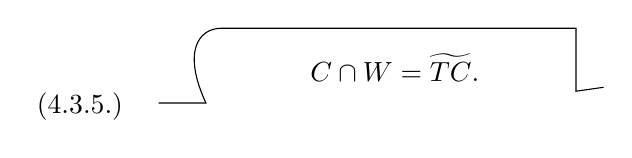
\begin{tikzpicture}
\node at (0,0) {$C\cap W=\widetilde{TC}.$};
\node at (-4,-0.5) {$(4.3.5.)$};
\draw (-3,-0.45)--(-2.4,-0.45).. controls (-2.7,0.2) and (-2.5,0.5)..(-2.2,0.5)--(2.3,0.5)--(2.3,-0.3)--(2.65,-0.25);
\end{tikzpicture}}
Dualement, si $\unsure{F|E},W$ sont stables par facteurs directs, les conditions équiv. de prop. 4.3. équivalent :
\[
F\cap W=\overline{TF}.
\tag*{(4.3.5')}
\]
En effet, si $C$ et $W$ sont stables par fact. directs, il en est de \unsure{$=$|même} de $C\cap W$, et \deleted{\unsure{comme}} dès lors si $C\cap W\subset\widetilde{TC}$, comme $C\cap W$ contient $TC$, \deleted{\unsure{donc}} on en déduit $\widetilde{C\cap W}=\widetilde{TC}$. Mais \deleted{\unsure{Comme} \unsure{et} $\unsure{C}$} Comme $C\cap W\unsure{\longleftrightarrow|\longleftarrow}TC$ et $C\cap W$ stable par facteurs directs, $C\cap W$ est clos : \unsure{i.e.} \deleted{\unsure{donc}} $C\cap W=\widetilde{C\cap W}$, par cor. 2 de prop. \unsure{4.2|4.3}, d'où $C\cap W=\widetilde{TC}$, qed.

\uline{Cor. 3} Supposons les conditions équivalentes \inserted{a) à c)} de prop. 4.3. satisfaites, et de plus \uline{$W$ stable par facteurs directs.}\textsuperscript{*} Alors les conditions préliminaires (4.3.1) et (4.3.2) restent satisfaites quand on remplace $(C,TF)$ et $(TC,F)$, par leurs clôtures \inserted{$(C',TF')=$} $(\unsure{\overline C|\widetilde C},\overline{TF})$ et \inserted{$(TC',F')=$} $(\widetilde{TC},\overline F)$, et les conditions \deleted{\unsure{analogues|équivalentes}} équivalentes de la prop. 4.3 sont \inserted{encore} satisfaites par ces couples, sous les formes \unsure{finales|fortes}
\[
\left\{\begin{aligned}
C'\cap W&=TC'\ (=\widetilde{TC}')\\
F'\cap W&=TF'\ (=\overline{TF}')\\
W&=TF'\circ TC'.
\end{aligned}\right.
\tag*{(4.3.6)}
\]
% margin note written slanted
\margin{* En fait, il suffit de supposer \unsure{que les|que l'on} \inserted{$W\supset\widetilde{TC},\overline{TF},$} \unsure{que tout|qui sont} facteur direct d'un élément de $W$ qui est soit dans $C$, soit dans $F$, est encore dans $W$. Alors $(\widetilde C,\widetilde{TC},\unsure{\overline F|\widetilde F},\overline{TF},W)$ définissent une structure de Q. close, et on sait \unsure{que ce|que cela} implique \unsure{qu'en|qu'un} fait, $W$ \unsure{est} lui aussi \unsure{stable} par facteurs directs (4.3.\unsure{6|5}).}
% archive sheet number: 160

\scanpage{162}\mspage{36}
Le triplet $(W,\unsure{E'|C'},F')$ est un triplet de Quillen clos (\unsure{correspondant|correspondent} : une ``closed model category'' de Quillen, \inserted{du moins} si on suppose $M$ stable par $\varinjlim$ finies et $\varprojlim$ finies, et que $W$ \deleted{\unsure{satisfait}} est \unsure{multiplicativement} saturé).

\uline{Démonstration} Les relations (4.3.1) impliquent
\[
\widetilde{TC}\subset\widetilde C\quad\text{et}\quad\overline{TF}\subset\overline F
\]
i.e.
\[
TC'\subset C',\quad TF'\subset F',
\]
i.e. (4.3.1) pour les nouveaux couples de Quillen. La relation 4.3.2. $W\supset TC,TF$, implique
\[
W\supset\widetilde{TC},\overline{TF},\quad\text{i.e.}\quad W\supset TC',TF'
\]
en vertu du cor. 2 à la prop. 4.2 et du fait que $W$ est stable par facteurs directs ; \deleted{\unsure{Comme}} donc on a (4.3.2) pour les nouveaux couples. Comme par hypothèse on a
\[
W=\overline{TF}\circ\widetilde{TC}
\]
ceci s'écrit
\[
W\unsure{\supset|=}TF'\circ TC',
\]
donc les nouveaux couples \unsure{satisfont} \unsure{aux} \unsure{$\Longrightarrow$|mêmes} conditions, qui cette fois, les couples étant clos, prennent la forme forte (4.3.6).

Prouvons que le triplet $(W,C',F')$ satisfait aux axiomes de Quillen d'une \deleted{structure} \inserted{triplet} de Quillen clos. On a bien, par 4.3.6.
\[
\left\{\begin{aligned}
C'&=\inserted{(TF')^*=}(F'\cap W)^*,\quad F'=(TC')_{\unsure{\alpha|*}}=(C'\cap W)_\alpha\\
W&=TF'\circ TC'=C'_*\circ F'^*
\end{aligned}\right.
\]
qui \unsure{correspondent|correspond} à la définition des \unsure{``|`}catégories de modèles de Quillen \uline{clos}\unsure{''|'} : les axiomes M1, \deleted{\unsure{les}} M2, M3, M4 de Quillen sont vérifiés de façon triviale, \deleted{M5 \unsure{par} \unsure{hyp.}} (M3 et M4 parce que

% margin note written sideways
\margin{Il en résulte le
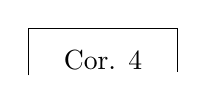
\begin{tikzpicture}\node at (0,0) {\uline{Cor. 4}};\draw (-0.95,-0.2)--(-0.95,0.4)--(0.95,0.4)--(0.95,-0.15);\end{tikzpicture}
\deleted{\unsure{Pour qu'un} \unsure{triplet} $(W,C,F)$ \unsure{soit} \unsure{un} \unsure{triplet}, de Quillen clos, il faut que \unsure{C clos} \unsure{et} \unsure{F clos}, \unsure{à droite}, $(C,TF\overset{\mathrm{def}}=\unsure{C_*})$ et $(TC\overset{\mathrm{def}}=C\cap W\unsure{)|,}$}
\inserted{\unsure{Soit} $W$ \unsure{un loc.} \unsure{mult.} \unsure{non multipli.|non vide|saturé},}
et $(C,TF),(TC,F)$ deux \unsure{précouples} de Quillen tels que $\unsure{TC|TE}\subset C\cap W$, $TF\subset F\cap W$, les cond. suivantes sont équiv.
\[
\begin{aligned}
\text{a)}\quad TC&=C\cap W\\
\text{b)}\quad TF&=F\cap W\\
\text{c)}\quad W&=TF\circ TC\\
\text{d)}\quad &(W,C,\unsure{P|F})\ \text{est un \unsure{triplet|couple}}\\
&\text{de Quillen clos.}
\end{aligned}
\]
}
% archive sheet number: 161

\scanpage{163}\mspage{37}
$C$ et $F$, $TC$ et $TF$ sont clos \unsure{à g.|: g.} \unsure{et} \unsure{resp.} à dr.). L'axiome M5 est la saturation \unsure{multiplicative} de $W$.
\figure{\begin{tikzpicture}\draw (0,0.4)--(0.4,0);\end{tikzpicture}}

\deleted{\unsure{5|\S|4}} \unsure{4.4.|44.} Voici l'idée pour construire $\pm$ ``toutes'' les \deleted{couples} structures de Quillen \unsure{closes|Closes|clos} $(C,TC,F,TF)$ \unsure{associée|associées} à un localiseur donné, $W\subset M$. On suppose que $M$ satisfait aux conditions du \S\ précédent, concernant l'existence de $\varinjlim$ filtrantes, d'une filtration cardinale, l'accessibilité de $M$ (\deleted{\unsure{en|et}}) \inserted{celle} des éléments de $\mathrm{Filt}^{\pi_0}$). On part d'une partie petite
\[
C_0\subset\mathrm{Fl}\,M
\]
telle que
\[
C_{0*}\subset W,
\tag*{(\deleted{\unsure{5}}4.4.1)}
\]
et on pose
\[
\left\{\begin{aligned}
C&=\widetilde C_0^{\unsure{.}},& TC&=C\cap W.\\
TF&=C_*=C_{0\unsure{\alpha|*|\bullet}},& F&=(TC)_*.
\end{aligned}\right.
\tag*{(4.4.2.)}
\]
\deleted{\unsure{On|Au}}

Il y a \deleted{deux} \inserted{un} \unsure{problèmes|problème} seulement \unsure{;|?} \unsure{vu} que l'on sait déjà que $(C,TF)$ est un couple de Quillen par le théorème de factorisation du \S\ 1 (p. \unsure{10|20}) : Il faut la factorisation pour le couple $(TC,F=(TC)_{\unsure{\alpha|*}})$. \unsure{À|A} ce moment là, les conditions préliminaires \inserted{(4.3.1) et (\unsure{4.3.2|4.3.1}) de prop.} 4.3. sont satisfaites $TC\subset C$, $TF\subset F$, $W\supset TC,TF$ \deleted{clos}, ainsi que la condition a $C\cap W\subset\widetilde{TC}$, puisque $C\cap W=TC$. Donc on trouve, par l'équivalence des conditions a, a', c) et vu que $TC$ et $TF$ sont clos
\[
TF=F\cap W,\quad W=TF\circ TC
\]
% archive sheet number: 162
